\documentclass[10pt,a4paper]{article}
\usepackage[utf8]{inputenc}
\usepackage[italian]{babel}
\usepackage{amsmath}
\usepackage{amsfonts}
\usepackage{amssymb}
\usepackage{graphicx}
\usepackage[left=2cm,right=2cm,top=2cm,bottom=2cm]{geometry}
\newcommand{\rem}[1]{[\emph{#1}]}
\newcommand{\exn}{\phantom{xxx}}
\renewcommand{\thesubsection}{\thesection.\alph{subsection}}  %% use 1.a numbering

\author{Gruppo 1G.BT \\ Francesco Sacco, Lorenzo Cavuoti}
\title{Es05B: Circuiti lineari con Amplificatori Operazionali}
\begin{document}
\date{8 Novembre 2018}
\maketitle


\section*{Scopo dell'~esperienza}
Misurare le caratteristiche di circuiti lineari realizzati con un op-amp TL081 alimentati tra +15 V e -15 V.

\section{Amplificatore invertente}
Si vuole realizzare un amplificatore invertente con un'~impedenza di ingresso superiore a 1 
k$\Omega$ e con un amplificazione a centro banda di 10.

\subsection{Scelta dei componenti}

Si monta il circuito secondo lo schema mostrato in figura \ref{fig:ampinv}, utilizzando la barra di 
distribuzione verde per la tensione negativa, quella rosso per la tensione positiva, e quella nera per 
la massa.

\rem{Indicare i criteri di scelta delle resistenze ed i valori desiderati}
%
\begin{figure}[h]
\begin{center}
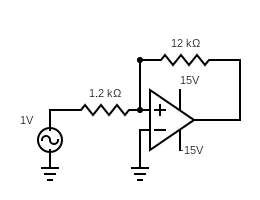
\includegraphics[width=0.4\linewidth]{circuit.png}
\caption{\small Schema di un amplificatore invertente}
\label{fig:ampinv}
\end{center}
\end{figure}
%

Le resistenze selezionate hanno i seguenti valori, misurati con il multimetro digitale, con il corrispondente valore atteso 
del guadagno in tensione dell'~amplificatore.
\[
R_1 = ( 1.19 \pm 0.01) \,\mathrm{k}\Omega, \quad 
R_2 = ( 12.2 \pm 0.1) \,\mathrm{k}\Omega, \quad 
A_{exp} = ( 10.2 \pm 0.1)
\]

\subsection{Montaggio circuito}

%%%%%%%%%%%%%%%%%%%%%%%%%%%%%%%%%%%%%%%%%%%%%%%%%%%%%%
\subsection{Linearit\`a e misura del guadagno}
Si fissa la frequenza del segnale ad $f_{in} = (5.59 \pm 0.06)$ kHz e si invia all'~ingresso dell'~amplificatore.
L'uscita dell'~amplificatore \`e mostrata qualitativativamente in Fig. \ref{fig:oscinv} per due 
differenti ampiezze di $V_{in}$ (circa $424mV$~Vpp e $4.32V$~Vpp). 
Nel primo caso l'~OpAmp si comporta in modo lineare mentre nel secondo caso si osserva clipping.   
%
\begin{figure}[h]
\begin{center}
\framebox(200,200){Screenshot oscillografo con $V_{out}$ lineare}
\framebox(200,200){Screenshot oscillografo con clipping di $V_{out}$}
%\includegraphics[0.45\textwidth]{}
%\includegraphics[0.45\textwidth]{}
\end{center}
\caption{\small Ingresso (in alto) ed uscita (in basso) di un amplificatore invertente con OpAmp, in 
zona lineare (a sinistra) e non (a destra)}
\label{fig:oscinv}
\end{figure}
%

Variando l'~ampiezza di $V_{in}$ si misura $V_{out}$ ed il relativo guadagno $A_V=V_{out}/V_{in}$ riportando i dati ottenuti in tabella~\ref{tab:guadagno} 
e mostrandone un grafico in Fig. \ref{fig:lin}. 

\begin{table}[h]
\caption{$V_{out}$ in funzione di $V_{in}$ e relativo rapporto.}
\label{tab:guadagno}
\begin{center}
\begin{tabular}{|c|c|c|}
\hline
$V_{in}$ (V) & $V_{out}$ (V)  & $A_V$ \\
\hline
\hline
$66 \pm 3\mathrm{m} $ & $680 \pm 30\mathrm{m} $ & $10.2 \pm 0.6 $ \\
\hline
$290 \pm 10\mathrm{m} $ & $2.9 \pm 0.1 $ & $10.1 \pm 0.6 $ \\
\hline
$730 \pm 30\mathrm{m} $ & $7.4 \pm 0.3 $ & $10.1 \pm 0.6 $ \\
\hline
$1.26 \pm 0.05 $ & $12.7 \pm 0.5 $ & $10.1 \pm 0.6 $ \\
\hline
$2.7 \pm 0.1 $ & $27 \pm 1 $ & $10 \pm 0.6 $ \\
\hline
\end{tabular}
\end{center}
\end{table}

\rem{Indicare in che modo si fa il fit, se sulla retta $V_{out}$ vs. $V_{in}$ oppure sui valori di $A_V$   }

Si determina il guadagno mediante fit dei dati ottenuti:
\[
A_{best} = 10.07 \pm 0.03 \quad  \chi^2 = 0.02
\]
\begin{figure}[t]
\begin{center}
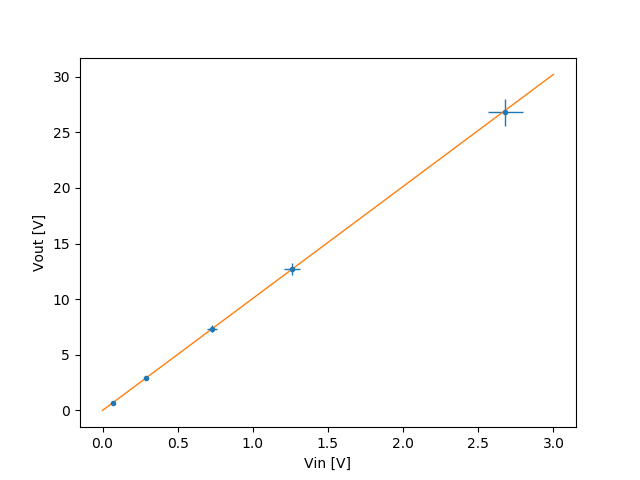
\includegraphics[width=0.8\linewidth]{1c.png}
\caption{\small Linearit\`a dell'~amplificatore invertente}
\label{fig:lin}
\end{center}
\end{figure}
%

\rem{Fino a quale tensione il circuito si comporta linearmente? Provare (facoltativamente) a ridurre la 
tensione di alimentazione dell'~integrato ed a verificarne la correlazione con la tensione di 
\emph{clipping} dell'~uscita. Commentare quanto osservato }

%%%%%%%%%%%%%%%%%%
%
\section{Risposta in frequenza e \emph{slew rate}}
\subsection{Risposta in frequenza del circuito}
Si misura la risposta in frequenza del circuito, riportando i dati  in Tab. \ref{tab:bodeinv} e
in un grafico di Bode in Fig. \ref{fig:bodeinv}, stimando la frequenza di taglio inferiore e 
superiore \rem{indicare in che modo}.
\[
V_{in} = (1.14 \pm 0.05 )\,\mathrm{V}
\]
\[
f_L = (7.5 \pm 0.3 )\,\mathrm{Hz}\;\;\;\;\;f_H = (210 \pm 4 \;)\,\mathrm{kHz}
\]
\begin{table}[h]
\caption{\small Guadagno dell'~amplificatore invertente in funzione della frequenza.}
\label{tab:bodeinv}
\begin{center}
\begin{tabular}{|c|c|c|}
\hline
$f_{in}$ (kHz) & $V_{out}$ (V) & $A$ (dB) \\
\hline
$2.58 \pm 0.3$& $ 3.8 \pm 0.2$& $3.3\pm 0.2$ \\ 
\hline
$172.0 \pm 2$& $ 11.6 \pm 0.5$& $10.2\pm 0.6$ \\
\hline
$5.56 \pm 0.06 k$& $ 11.5 \pm 0.5$& $10.1\pm 0.6$ \\ 
\hline
$67.7 \pm 0.7 k$& $ 11.0 \pm 0.5$& $9.6\pm 0.6$ \\ 
\hline
$952 \pm 10 k$& $ 2.5 \pm 0.1$& $2.2\pm 0.1$ \\ 
\hline
\end{tabular}
\end{center}
\end{table} 




 


\begin{figure}[h]
\begin{center}
\framebox(200,200){Inserire plot di Bode dell'~invertente.}
%\includegraphics[width=0.7\textwidth]{}
\caption{\small Plot di Bode in ampiezza per l'~amplificatore invertente.}
\label{fig:bodeinv}
\end{center}
\end{figure}
%
\subsection{Misura dello \emph{slew-rate}}
Si misura direttamente lo \emph{slew-rate} dell'op-amp inviando in ingresso un'~onda quadra 
di frequenza di $\sim 2.11$~kHz e di ampiezza $\sim 2.70$~V. Si ottiene:
\[
SR_\mathrm{misurato} = (7.7 \pm 0.3 )\,\mathrm{V/\mu s} \quad \mathrm{valore \; tipico}\, (\exn )\,\mathrm{V/\mu s}\
\]

\rem{Commentare accordo o disaccordo. Eventualmente inserire screenshot dell'oscilloscopio}
%
\section{Circuito integratore}
Si monta il circuito integratore con i seguenti valori  dei componenti indicati: 
\[
R_1 = (0.990 \pm  0.008\;) \,\mathrm{k}\Omega, \:\:\;\:\exn 
R_2 = (9.83 \pm 0.08 \;) \,\mathrm{k}\Omega, \:\:\;\:\exn 
C = (\;49 \pm 2 \;\;)\,\mathrm{nF}
\]

\subsection{Risposta in frequenza}

Si invia un'~onda sinusoidale e si misura la risposta in frequenza dell'~amplificazione e della fase riportandoli 
nella tabella \ref{tab:bodeinte} e in un diagramma di Bode in Fig. \ref{fig:bodeinte}. 
\[
V_{in} = (1.03 \pm 0.04 )\,\mathrm{V}
\]
\rem{La fase pu\'o essere indicata in gradi, radianti, oppure come frazione $\phi/2\pi$}
%
\begin{table}[h]
\caption{Guadagno e fase dell'~integratore invertente in funzione della frequenza.}
\label{tab:bodeinte}
\begin{center}
\begin{tabular}{|c|c|c|c|c|}
\hline
$f_{in}$ (kHz) & $V_{out}$ (V) & $A$ (dB) & $\Delta t (\mu s)$ & $\phi$ \\
\hline
$\exn \pm \exn $ & $\exn \pm \exn $ & $\exn \pm \exn $ & $\exn \pm \exn $ & $\exn \pm \exn $ \\
\hline
$\exn \pm \exn $ & $\exn \pm \exn $ & $\exn \pm \exn $ & $\exn \pm \exn $ & $\exn \pm \exn $ \\
\hline
$\exn \pm \exn $ & $\exn \pm \exn $ & $\exn \pm \exn $ & $\exn \pm \exn $ & $\exn \pm \exn $ \\
\hline
$\exn \pm \exn $ & $\exn \pm \exn $ & $\exn \pm \exn $ & $\exn \pm \exn $ & $\exn \pm \exn $ \\
\hline
$\exn \pm \exn $ & $\exn \pm \exn $ & $\exn \pm \exn $ & $\exn \pm \exn $ & $\exn \pm \exn $ \\
\hline
$\exn \pm \exn $ & $\exn \pm \exn $ & $\exn \pm \exn $ & $\exn \pm \exn $ & $\exn \pm \exn $ \\
\hline
$\exn \pm \exn $ & $\exn \pm \exn $ & $\exn \pm \exn $ & $\exn \pm \exn $ & $\exn \pm \exn $ \\
\hline
\end{tabular}
\end{center}
\end{table} 
%
\begin{figure}[htb]
\begin{center}
\framebox(200,200){Inserire plot di Bode in ampiezza}
\framebox(200,200){Analogo in fase}
%\includegraphics[0.45\textwidth]{}
%\includegraphics[0.45\textwidth]{}
\end{center}
\caption{\small Plot di Bode in ampiezza (a sinistra) e fase (a destra) per il circuito integratore.}
\label{fig:bodeinte}
\end{figure}
%

Si ricava una stima delle caratteristiche principali dell'andamento (guadagno a bassa frequenza, frequenza di taglio, e pendenza ad alta frequenza)
e si confrontano con quanto atteso. Non si effettua la stima degli errori, trattandosi di misure qualitative.

\rem{Indicare brevemente come sono stati ottenuti i valori attesi}

\begin{align*}
A_M &= (9.5)\,\mathrm{dB} & \mathrm{atteso} &:\,(\exn  )\, \mathrm{dB}  \\
f_H &= (355)\,\mathrm{Hz} & \mathrm{atteso} &:\,(\exn  )\, \mathrm{Hz} \\
{\mathrm{d}A_V}/{\mathrm{d}f} &= (18.6)\,\mathrm{dB/decade} & \mathrm{atteso} &:\,(\exn  )\, \mathrm{dB/decade}  \\
\end{align*}


%
\subsection*{Risposta ad un'~onda quadra}
Si invia all'~ingresso un'~onda quadra di frequenza $\sim 6.47\,kHz$ e ampiezza $\sim 1.09\,V$.
Si riporta in Fig. \ref{fig:oscinte} le forme d'~onda acquisite all'~oscillografo per l'~ingresso
e l'~uscita. 

\rem{Commentare se che il circuito si comporta come un integratore.}
%
\begin{figure}[htb]
\begin{center}
\framebox(200,200){Inserire screenshot oscillografo per integratore}
%\includegraphics[0.45\textwidth]{}
\end{center}
\caption{\small Ingresso (in alto) ed uscita (in basso) del circuito integratore per un'~onda quadra.}
\label{fig:oscinte}
\end{figure}
%

Si misura l'~ampiezza dell'~onda  in uscita e si confronta il valore atteso.

\rem{Indicare brevemente come sono stati ottenuti i valori attesi}
\begin{align*}
V_{out} &= (0.86 )\,\mathrm{V} & \mathrm{atteso} &:\,(\exn  )\, \mathrm{V}  \\
\end{align*}

\rem{Inserire commento sulla dipendenza dell'~uscita dalla frequenza.}
%

\subsection{Discussione}

\rem{Inserire commenti su quanto osservato ed eventuali deviazioni. 
In particolare: attenuazione ad alte frequenze, dipendenza della fase dalla frequenza, funzione di $R_2$. }

%%%%%%%%%%%%%%%%%%%%%%%%

\end{document}          
